\begin{figure}[H]
\centering
\resizebox{0.80\linewidth}{!}{%
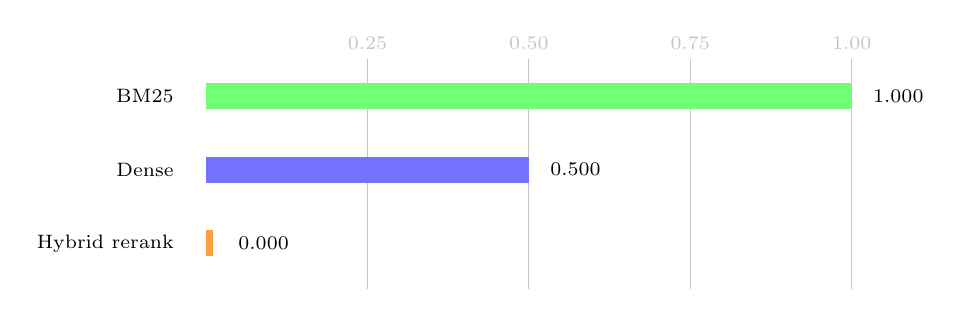
\begin{tikzpicture}[x=8.2cm,y=0.72cm,font=\scriptsize]
\foreach \x/\lab in {0.25/0.25,0.50/0.50,0.75/0.75,1.00/1.00}
  \draw[gray!45] (\x,0.55) -- (\x,4.60) node[above]{\lab};

\node[anchor=east] at (-0.035,3.95) {BM25};
\fill[green!55] (0,3.72) rectangle (1.00,4.18);
\node[anchor=west] at (1.018,3.95) {1.000};

\node[anchor=east] at (-0.035,2.65) {Dense};
\fill[blue!55] (0,2.42) rectangle (0.50,2.88);
\node[anchor=west] at (0.518,2.65) {0.500};

\node[anchor=east] at (-0.035,1.35) {Hybrid rerank};
\fill[orange!75] (0,1.12) rectangle (0.01,1.58);
\node[anchor=west] at (0.035,1.35) {0.000};
\end{tikzpicture}
}
\caption{Section 6 ablation hit rate at top-$k=3$ over two benchmark questions. In this small measured run, BM25 recovered both gold cases, dense recovered one, and hybrid rerank recovered none.}
\label{fig:section6-ablation}
\end{figure}
